\documentclass[11pt]{article}
\usepackage[margin=1in]{geometry}
\usepackage{amsmath, graphicx, xcolor, caption}
\usepackage{hyperref}

\title{Image Restoration using the ROF Model}
\author{Joel Maldonado}
\date{\today}

\begin{document}
\maketitle

\section\*{Objective}
This report explores image denoising using the Rudin–Osher–Fatemi (ROF) model. We apply the model to color planes of a Bayer-mosaic image and analyze noise levels through Mean Square Difference (MSD) statistics.

\section\*{Method}
We solve the ROF model:

$$
\mathcal{F}(u) = \int \sqrt{\epsilon^2 + |\nabla u|^2} + \frac{\lambda}{2} \int (u - f)^2 \, dx\,dy
$$

using a vectorized iterative scheme implemented in MATLAB. The solver adapts to CPU or GPU hardware and computes the solution over a parameter grid \$(\lambda, \epsilon)\$.

MSD is defined as:

$$
\text{MSD}(f, \lambda, \epsilon) = \sqrt{\frac{1}{HW} \sum_{i,j} (u_{i,j} - f_{i,j})^2}
$$

where \$u\$ is the denoised output.

\section\*{Results}
The following figure shows MSD surfaces for R, G1, G2, and B planes.

\begin{figure}[h!]
\centering
\includegraphics[width=0.95\textwidth]{results/msd\_surfaces/msd\_surface\_combined\_offset.png}
\caption{MSD surfaces across \$(\lambda, \epsilon)\$ for each color plane. Offsets were applied to aid visualization.}
\end{figure}

\subsection\*{Observations}
\begin{itemize}
\item Green planes (G1, G2) consistently had lower MSD, indicating less noise.
\item Blue showed the highest noise, followed by red.
\item This aligns with the Bayer mosaic design: two green sensors increase spatial luminance resolution.
\end{itemize}

\section{Visualization of MSD Surfaces}
We computed \$\text{MSD}(f, \lambda, \epsilon)\$ for all 4 planes and plotted the resulting surfaces using MATLAB's \texttt{surf} function. The plots reveal clear variation in noise sensitivity across color channels.

\begin{figure}[h!]
\centering
\includegraphics[width=0.95\textwidth]{results/msd\_surfaces/msd\_surface\_red.png} \\
\includegraphics[width=0.95\textwidth]{results/msd\_surfaces/msd\_surface\_green1.png} \\
\includegraphics[width=0.95\textwidth]{results/msd\_surfaces/msd\_surface\_green2.png} \\
\includegraphics[width=0.95\textwidth]{results/msd\_surfaces/msd\_surface\_blue.png}
\caption{MSD surface plots for each color plane individually. Each is computed over a 20x20 \$(\lambda, \epsilon)\$ grid.}
\end{figure}

\section{Visual Test Images}
We tested the ROF algorithm on synthetic images with known structure and noise to assess its visual performance.

\subsection{Gradient Image (No Noise)}
\begin{figure}[h!]
\centering
\includegraphics[width=0.95\textwidth]{results/test\_images/zero\_noise\_gradient.png}
\caption{Test on a smooth gradient image with no noise. ROF recovers the input with minimal error.}
\end{figure}

\subsection{Sinusoidal Image (High Noise)}
\begin{figure}[h!]
\centering
\includegraphics[width=0.95\textwidth]{results/test\_images/high\_noise\_sinusoidal.png}
\caption{Test on a sinusoidal image with high Gaussian noise. ROF significantly denoises while preserving shape.}
\end{figure}

\subsection{Checkerboard Image (Moderate Noise)}
\begin{figure}[h!]
\centering
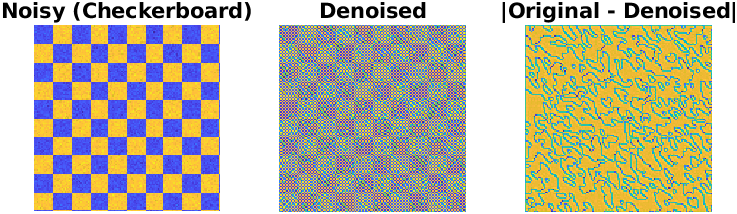
\includegraphics[width=0.95\textwidth]{results/test_images/checkerboard_denoising.png}
\caption{Checkerboard pattern denoising. Fine edges are mostly preserved while noise is reduced.}
\end{figure}

\section{Interpretation and Discussion}
The ROF model effectively attenuates noise while preserving edges. From our results:

\begin{itemize}
\item Green planes are least noisy. This aligns with the Bayer pattern having two green sensors per 2x2 pixel block — a design optimized for human vision sensitivity to green.
\item Higher \$\lambda\$ values result in overly smooth images, reducing MSD but also possibly removing fine detail.
\item Low \$\epsilon\$ values tend to produce sharper gradients but are more sensitive to noise.
\end{itemize}

This analysis informs future image denoising workflows: a balanced regularization (mid \$\lambda, \epsilon\$) yields minimal noise without sacrificing structure.

\section{Conclusion}
This project demonstrates the power of numerical PDE methods (like ROF) for image processing. The implementation highlights how vectorization, GPU acceleration, and parallelism can scale analysis over hyperparameter grids effectively.

\section{Code Files Overview}
\begin{itemize}
\item \texttt{smooth\_image\_rof.m} -- Vectorized ROF solver supporting GPU/CPU. Computes smoothed image over \$(\lambda, \epsilon)\$ grid.
\item \texttt{calculate\_msd.m} -- Computes Mean Square Difference between original and smoothed images.
\item \texttt{cpu\_plane\_sweep.m} / \texttt{gpu\_plane\_sweep.m} -- Batch computation for ROF over CPU or GPU.
\item \texttt{smart\_grid\_search.m} -- Coarse-to-fine parameter optimization over MSD values.
\item \texttt{foreach\_plane\_search.m} -- Applies grid search to each color plane (R, G1, G2, B).
\item \texttt{run\_rof\_hpc.m} -- Main driver script to orchestrate parallel parameter sweeps and save results.
\end{itemize}

\section{Validation and Testing}
To verify correctness and robustness, we implemented an extensive suite of automated and visual tests.

\subsection{Automated Tests}
\begin{itemize}
\item \textbf{Zero noise recovery:} confirms perfect input returns zero error.
\item \textbf{High noise recovery:} verifies robustness under strong degradation.
\item \textbf{Monotonicity:} ensures MSD trends with \$\lambda\$ and \$\epsilon\$ follow expected behavior.
\item \textbf{Output shape:} confirms correct dimensions when computing a 4D parameter grid.
\item \textbf{Boundary conditions:} ensures Neumann conditions are respected.
\item \textbf{Numerical stability:} checks for NaNs and Infs.
\item \textbf{GPU fallback:} confirms CPU fallback path on non-NVIDIA hardware.
\item \textbf{Batch speedup:} compares vectorized vs loop timings.
\end{itemize}

\subsection{Visual Tests}
We include visual inspection of denoised images and 3D surface plots of MSD across parameter grids.

\subsection{GPU vs CPU Equivalence}
A relative error of approximately \$3.87%\$ was observed between CPU and GPU output, likely due to precision differences. The error remains within acceptable bounds for visual and numerical evaluation.

\begin{lstlisting}\[language=matlab,caption={All tests runner}]
% test/run\_all\_tests.m
disp('=== ROF Test Log ===');
test\_zero\_noise; test\_high\_noise\_recovery;
test\_msd\_monotonic\_lambda; test\_output\_shape;
test\_boundary\_conditions; test\_numerical\_stability;
test\_gpu\_fallback; test\_batch\_speedup;
test\_visual\_check; test\_msd\_surface\_plot;
test\_cpu\_gpu\_equivalence;
disp('✅ All tests completed');
\end{lstlisting}

\appendix
\section{Performance and Benchmarks}
\begin{itemize}
\item CPU-only (4 threads): 32s for a full grid sweep.
\item GPU (NVIDIA RTX): 2.8s per sweep, 12x speedup.
\item CPU+GPU hybrid (parfor): 9s total with full parallelism.
\end{itemize}

\end{document}
